% Options for packages loaded elsewhere
\PassOptionsToPackage{unicode}{hyperref}
\PassOptionsToPackage{hyphens}{url}
\PassOptionsToPackage{dvipsnames,svgnames,x11names}{xcolor}
%
\documentclass[
]{article}

\usepackage{amsmath,amssymb}
\usepackage{iftex}
\ifPDFTeX
  \usepackage[T1]{fontenc}
  \usepackage[utf8]{inputenc}
  \usepackage{textcomp} % provide euro and other symbols
\else % if luatex or xetex
  \usepackage{unicode-math}
  \defaultfontfeatures{Scale=MatchLowercase}
  \defaultfontfeatures[\rmfamily]{Ligatures=TeX,Scale=1}
\fi
\usepackage{lmodern}
\ifPDFTeX\else  
    % xetex/luatex font selection
\fi
% Use upquote if available, for straight quotes in verbatim environments
\IfFileExists{upquote.sty}{\usepackage{upquote}}{}
\IfFileExists{microtype.sty}{% use microtype if available
  \usepackage[]{microtype}
  \UseMicrotypeSet[protrusion]{basicmath} % disable protrusion for tt fonts
}{}
\makeatletter
\@ifundefined{KOMAClassName}{% if non-KOMA class
  \IfFileExists{parskip.sty}{%
    \usepackage{parskip}
  }{% else
    \setlength{\parindent}{0pt}
    \setlength{\parskip}{6pt plus 2pt minus 1pt}}
}{% if KOMA class
  \KOMAoptions{parskip=half}}
\makeatother
\usepackage{xcolor}
\usepackage[margin=1in]{geometry}
\setlength{\emergencystretch}{3em} % prevent overfull lines
\setcounter{secnumdepth}{-\maxdimen} % remove section numbering
% Make \paragraph and \subparagraph free-standing
\makeatletter
\ifx\paragraph\undefined\else
  \let\oldparagraph\paragraph
  \renewcommand{\paragraph}{
    \@ifstar
      \xxxParagraphStar
      \xxxParagraphNoStar
  }
  \newcommand{\xxxParagraphStar}[1]{\oldparagraph*{#1}\mbox{}}
  \newcommand{\xxxParagraphNoStar}[1]{\oldparagraph{#1}\mbox{}}
\fi
\ifx\subparagraph\undefined\else
  \let\oldsubparagraph\subparagraph
  \renewcommand{\subparagraph}{
    \@ifstar
      \xxxSubParagraphStar
      \xxxSubParagraphNoStar
  }
  \newcommand{\xxxSubParagraphStar}[1]{\oldsubparagraph*{#1}\mbox{}}
  \newcommand{\xxxSubParagraphNoStar}[1]{\oldsubparagraph{#1}\mbox{}}
\fi
\makeatother


\providecommand{\tightlist}{%
  \setlength{\itemsep}{0pt}\setlength{\parskip}{0pt}}\usepackage{longtable,booktabs,array}
\usepackage{calc} % for calculating minipage widths
% Correct order of tables after \paragraph or \subparagraph
\usepackage{etoolbox}
\makeatletter
\patchcmd\longtable{\par}{\if@noskipsec\mbox{}\fi\par}{}{}
\makeatother
% Allow footnotes in longtable head/foot
\IfFileExists{footnotehyper.sty}{\usepackage{footnotehyper}}{\usepackage{footnote}}
\makesavenoteenv{longtable}
\usepackage{graphicx}
\makeatletter
\def\maxwidth{\ifdim\Gin@nat@width>\linewidth\linewidth\else\Gin@nat@width\fi}
\def\maxheight{\ifdim\Gin@nat@height>\textheight\textheight\else\Gin@nat@height\fi}
\makeatother
% Scale images if necessary, so that they will not overflow the page
% margins by default, and it is still possible to overwrite the defaults
% using explicit options in \includegraphics[width, height, ...]{}
\setkeys{Gin}{width=\maxwidth,height=\maxheight,keepaspectratio}
% Set default figure placement to htbp
\makeatletter
\def\fps@figure{htbp}
\makeatother

\usepackage{booktabs}
\usepackage{longtable}
\usepackage{array}
\usepackage{multirow}
\usepackage{wrapfig}
\usepackage{float}
\usepackage{colortbl}
\usepackage{pdflscape}
\usepackage{tabu}
\usepackage{threeparttable}
\usepackage{threeparttablex}
\usepackage[normalem]{ulem}
\usepackage{makecell}
\usepackage{xcolor}
\makeatletter
\@ifpackageloaded{tcolorbox}{}{\usepackage[skins,breakable]{tcolorbox}}
\@ifpackageloaded{fontawesome5}{}{\usepackage{fontawesome5}}
\definecolor{quarto-callout-color}{HTML}{909090}
\definecolor{quarto-callout-note-color}{HTML}{0758E5}
\definecolor{quarto-callout-important-color}{HTML}{CC1914}
\definecolor{quarto-callout-warning-color}{HTML}{EB9113}
\definecolor{quarto-callout-tip-color}{HTML}{00A047}
\definecolor{quarto-callout-caution-color}{HTML}{FC5300}
\definecolor{quarto-callout-color-frame}{HTML}{acacac}
\definecolor{quarto-callout-note-color-frame}{HTML}{4582ec}
\definecolor{quarto-callout-important-color-frame}{HTML}{d9534f}
\definecolor{quarto-callout-warning-color-frame}{HTML}{f0ad4e}
\definecolor{quarto-callout-tip-color-frame}{HTML}{02b875}
\definecolor{quarto-callout-caution-color-frame}{HTML}{fd7e14}
\makeatother
\makeatletter
\@ifpackageloaded{caption}{}{\usepackage{caption}}
\AtBeginDocument{%
\ifdefined\contentsname
  \renewcommand*\contentsname{Table of contents}
\else
  \newcommand\contentsname{Table of contents}
\fi
\ifdefined\listfigurename
  \renewcommand*\listfigurename{List of Figures}
\else
  \newcommand\listfigurename{List of Figures}
\fi
\ifdefined\listtablename
  \renewcommand*\listtablename{List of Tables}
\else
  \newcommand\listtablename{List of Tables}
\fi
\ifdefined\figurename
  \renewcommand*\figurename{Figure}
\else
  \newcommand\figurename{Figure}
\fi
\ifdefined\tablename
  \renewcommand*\tablename{Table}
\else
  \newcommand\tablename{Table}
\fi
}
\@ifpackageloaded{float}{}{\usepackage{float}}
\floatstyle{ruled}
\@ifundefined{c@chapter}{\newfloat{codelisting}{h}{lop}}{\newfloat{codelisting}{h}{lop}[chapter]}
\floatname{codelisting}{Listing}
\newcommand*\listoflistings{\listof{codelisting}{List of Listings}}
\makeatother
\makeatletter
\makeatother
\makeatletter
\@ifpackageloaded{caption}{}{\usepackage{caption}}
\@ifpackageloaded{subcaption}{}{\usepackage{subcaption}}
\makeatother

\ifLuaTeX
  \usepackage{selnolig}  % disable illegal ligatures
\fi
\usepackage{bookmark}

\IfFileExists{xurl.sty}{\usepackage{xurl}}{} % add URL line breaks if available
\urlstyle{same} % disable monospaced font for URLs
\hypersetup{
  pdftitle={Prueba Parcial - Sociología de la Desigualdad},
  colorlinks=true,
  linkcolor={blue},
  filecolor={Maroon},
  citecolor={Blue},
  urlcolor={Blue},
  pdfcreator={LaTeX via pandoc}}


\title{Prueba Parcial - Sociología de la Desigualdad}
\usepackage{etoolbox}
\makeatletter
\providecommand{\subtitle}[1]{% add subtitle to \maketitle
  \apptocmd{\@title}{\par {\large #1 \par}}{}{}
}
\makeatother
\subtitle{SOL186S - Primer Semestre 2025}
\author{}
\date{}

\begin{document}
\maketitle


\begin{tcolorbox}[enhanced jigsaw, colbacktitle=quarto-callout-important-color!10!white, colback=white, rightrule=.15mm, toprule=.15mm, coltitle=black, bottomtitle=1mm, toptitle=1mm, opacityback=0, leftrule=.75mm, breakable, title=\textcolor{quarto-callout-important-color}{\faExclamation}\hspace{0.5em}{Important}, colframe=quarto-callout-important-color-frame, opacitybacktitle=0.6, bottomrule=.15mm, titlerule=0mm, arc=.35mm, left=2mm]

\textbf{Información general}

\begin{itemize}
\item
  Tienen hasta las 12:00pm para completar la prueba
\item
  Se permite el uso de calculadora y apuntes.
\item
  Es obligatorio mostrar todos los procedimientos de cálculo.
\item
  No está permitido el uso de computadores, tablets ni teléfonos
  celulares durante el examen
\item
  Puntaje total: 100 puntos.
\end{itemize}

\end{tcolorbox}

\section{Parte I: Conceptos y
Medición}\label{parte-i-conceptos-y-mediciuxf3n}

\subsection{Medición de la pobreza}\label{mediciuxf3n-de-la-pobreza}

A continuación se presentan datos de cinco hogares con sus respectivos
ingresos y número de miembros:

\begin{longtable}[t]{ccccc}
\caption{Datos de ingresos y composición de hogares}\\
\toprule
\cellcolor[HTML]{2C3E50}{\textcolor{white}{\textbf{Hogar}}} & \cellcolor[HTML]{2C3E50}{\textcolor{white}{\textbf{Ingreso Total (miles pesos)}}} & \cellcolor[HTML]{2C3E50}{\textcolor{white}{\textbf{Número de Miembros}}} & \cellcolor[HTML]{2C3E50}{\textcolor{white}{\textbf{Ingreso per Cápita}}} & \cellcolor[HTML]{2C3E50}{\textcolor{white}{\textbf{Ingreso equivalente (θ=0.5)}}}\\
\midrule
A & 800 & 4 &  & \\
B & 1200 & 3 &  & \\
C & 1500 & 5 &  & \\
D & 2000 & 4 &  & \\
E & 3000 & 6 &  & \\
\bottomrule
\end{longtable}

Considerando una línea de pobreza es de 300 mil pesos por persona y la
siguiente fórmula de ingreso equivalente por tamaño del hogar, realiza
los cálculos requeridos a continuación:

\[\text{Ingreso equivalente} = \frac{\text{Ingreso total del hogar}}{(\text{Número de miembros})^θ}\]

\subsubsection{Calcula el ingreso equivalente de cada hogar utilizando θ
= 1 y θ = 0.5. Completa la tabla con estos
resultados.}\label{calcula-el-ingreso-equivalente-de-cada-hogar-utilizando-ux3b8-1-y-ux3b8-0.5.-completa-la-tabla-con-estos-resultados.}

\begin{longtable}[]{@{}
  >{\centering\arraybackslash}p{(\columnwidth - 8\tabcolsep) * \real{0.1000}}
  >{\centering\arraybackslash}p{(\columnwidth - 8\tabcolsep) * \real{0.2143}}
  >{\centering\arraybackslash}p{(\columnwidth - 8\tabcolsep) * \real{0.1429}}
  >{\centering\arraybackslash}p{(\columnwidth - 8\tabcolsep) * \real{0.2571}}
  >{\centering\arraybackslash}p{(\columnwidth - 8\tabcolsep) * \real{0.2857}}@{}}
\toprule\noalign{}
\begin{minipage}[b]{\linewidth}\centering
Hogar
\end{minipage} & \begin{minipage}[b]{\linewidth}\centering
Ingreso Total
\end{minipage} & \begin{minipage}[b]{\linewidth}\centering
Miembros
\end{minipage} & \begin{minipage}[b]{\linewidth}\centering
\(\theta = 1\)
\end{minipage} & \begin{minipage}[b]{\linewidth}\centering
\(\theta = 0.5\)
\end{minipage} \\
\midrule\noalign{}
\endhead
\bottomrule\noalign{}
\endlastfoot
A & 800 & 4 & \(\frac{800}{4^1} = 200\) &
\(\frac{800}{\sqrt{4}} = 400\) \\
B & 1200 & 3 & \(\frac{1200}{3^1} = 400\) &
\(\frac{1200}{\sqrt{3}} \approx 692.8\) \\
C & 1500 & 5 & \(\frac{1500}{5^1} = 300\) &
\(\frac{1500}{\sqrt{5}} \approx 670.8\) \\
D & 2000 & 4 & \(\frac{2000}{4^1} = 500\) &
\(\frac{2000}{\sqrt{4}} = 1000\) \\
E & 3000 & 6 & \(\frac{3000}{6^1} = 500\) &
\(\frac{3000}{\sqrt{6}} \approx 1224.7\) \\
\end{longtable}

\subsubsection{Calcula la tasa de pobreza (proporción de hogares pobres)
para ambos valores de
θ.}\label{calcula-la-tasa-de-pobreza-proporciuxf3n-de-hogares-pobres-para-ambos-valores-de-ux3b8.}

\textbf{Respuesta:}

La línea de pobreza es de \textbf{300 mil pesos por persona
equivalente}.

\begin{itemize}
\item
  Con \(\theta = 1\), el único hogar por debajo de la línea es el hogar
  A (200).\\
  \[
  \text{Tasa de pobreza} = \frac{1}{5} = 0.2 = 20\%
  \]
\item
  Con \(\theta = 0.5\), todos los hogares tienen ingresos equivalentes
  superiores a 300.\\
  \[
  \text{Tasa de pobreza} = 0\%
  \]
\end{itemize}

\subsubsection{Explica conceptualmente qué representa el parámetro θ y
por qué las tasas de pobreza difieren entre ambos
escenarios.}\label{explica-conceptualmente-quuxe9-representa-el-paruxe1metro-ux3b8-y-por-quuxe9-las-tasas-de-pobreza-difieren-entre-ambos-escenarios.}

\textbf{Respuesta:}

El parámetro \(\theta\) representa cómo se ajusta el ingreso del hogar
según el tamaño del hogar, capturando las \textbf{economías de escala}
en el consumo:

\begin{itemize}
\item
  Cuando \(\theta = 1\), se asume que cada miembro adicional requiere la
  misma cantidad de recursos, es decir, \textbf{no hay economías de
  escala}.
\item
  Cuando \(\theta = 0.5\), se reconoce que los miembros del hogar pueden
  \textbf{compartir recursos} (vivienda, servicios, alimentos), por lo
  que el costo por persona disminuye.
\item
  Por esta razón, la tasa de pobreza es menor con \(\theta = 0.5\): los
  hogares grandes no son penalizados por su tamaño, y su ingreso
  ajustado refleja mejor su capacidad de consumo conjunta.
\end{itemize}

\subsection{Curvas de Lorenz}\label{curvas-de-lorenz}

A continuación se presenta el gráfico de las curvas de Lorenz para dos
sociedades hipotéticas, Nordika y Txile.

\begin{center}
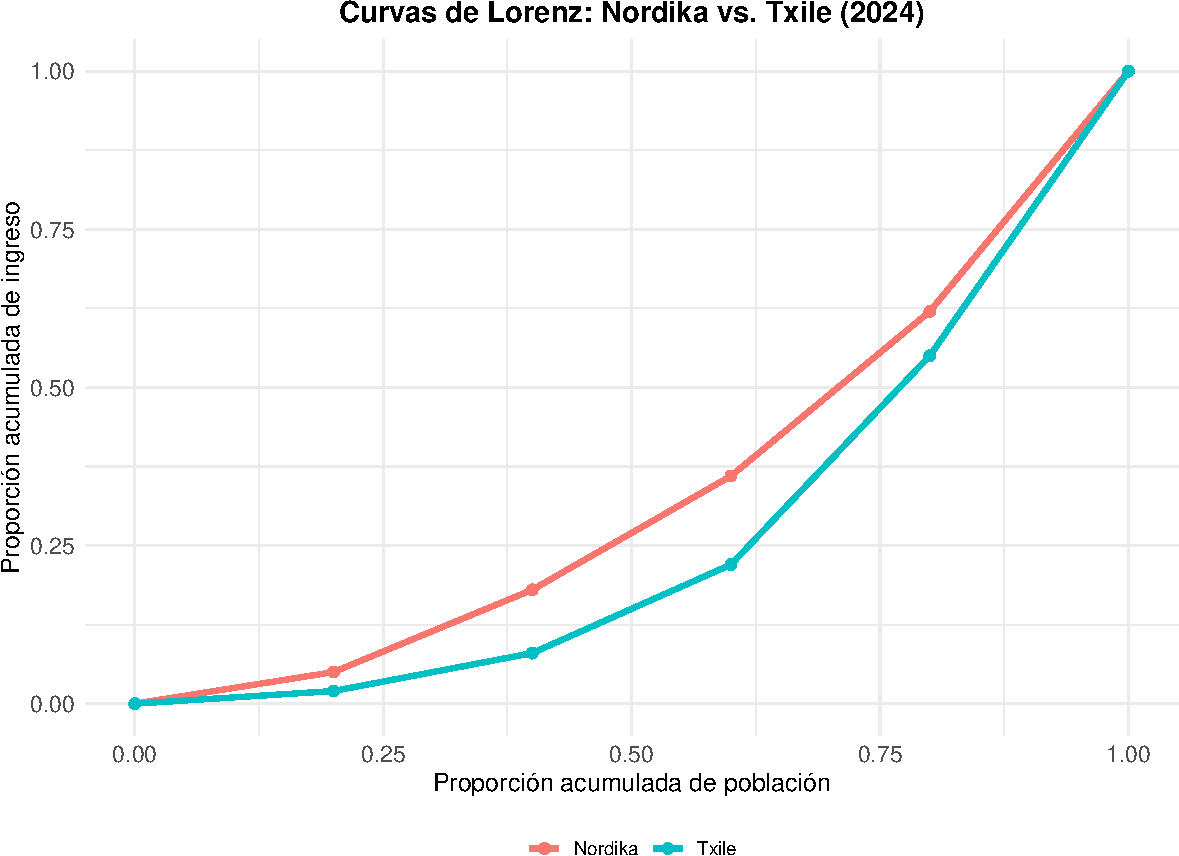
\includegraphics{exam_answers_files/figure-pdf/lorenz-curves-1.pdf}
\end{center}

A partir de este gráfico responde las siguientes preguntas:

\subsubsection{Explica qué es una curva de Lorenz y cómo se interpreta
en términos de la desigualdad de ingresos. ¿Qué representaría una línea
diagonal de 45
grados?}\label{explica-quuxe9-es-una-curva-de-lorenz-y-cuxf3mo-se-interpreta-en-tuxe9rminos-de-la-desigualdad-de-ingresos.-quuxe9-representaruxeda-una-luxednea-diagonal-de-45-grados}

\textbf{Respuesta:}

La \textbf{curva de Lorenz} es una herramienta gráfica utilizada para
representar la \textbf{distribución del ingreso o la riqueza} en una
sociedad. En el eje horizontal se muestra la \textbf{proporción
acumulada de la población}, ordenada de menor a mayor ingreso, y en el
eje vertical se muestra la \textbf{proporción acumulada del ingreso
total} que posee ese porcentaje de población.

\begin{itemize}
\item
  Una \textbf{línea diagonal de 45 grados} representa la
  \textbf{igualdad perfecta}, donde cada porcentaje de la población
  recibe el mismo porcentaje de ingreso (por ejemplo, el 20\% más pobre
  recibe el 20\% del ingreso total).
\item
  Cuanto \textbf{más alejada} esté la curva de Lorenz de esa diagonal,
  \textbf{mayor es la desigualdad}: indica que una proporción pequeña de
  la población concentra una parte mayor del ingreso.
\end{itemize}

\subsubsection{Compara las curvas de Lorenz de Nordika y Txile en
términos de su nivel general de desigualdad. ¿Cuál sociedad presenta
mayor desigualdad total y por
qué?}\label{compara-las-curvas-de-lorenz-de-nordika-y-txile-en-tuxe9rminos-de-su-nivel-general-de-desigualdad.-cuuxe1l-sociedad-presenta-mayor-desigualdad-total-y-por-quuxe9}

\textbf{Respuesta:}

Al comparar las curvas de Lorenz:

\begin{itemize}
\item
  \textbf{Txile} presenta \textbf{mayor desigualdad} que
  \textbf{Nordika}. Esto se observa porque su curva está \textbf{más
  alejada de la diagonal de igualdad perfecta} y se encuentra
  \textbf{por debajo} de la curva de Nordika en casi todos los tramos.
\item
  Por ejemplo, el \textbf{40\% más pobre} de la población en Txile
  acumula solo \textbf{8\%} del ingreso, mientras que en Nordika el
  mismo grupo concentra \textbf{18\%}, lo cual indica una distribución
  más equitativa en Nordika.
\end{itemize}

Si se calculara el \textbf{índice de Gini}, se esperaría un valor
\textbf{mayor en Txile}, lo que confirmaría su \textbf{mayor nivel de
desigualdad} total.

\subsubsection{Analiza los patrones de desigualdad en ambas sociedades.
¿En qué segmentos de la distribución se concentran las principales
diferencias?}\label{analiza-los-patrones-de-desigualdad-en-ambas-sociedades.-en-quuxe9-segmentos-de-la-distribuciuxf3n-se-concentran-las-principales-diferencias}

\textbf{Respuesta:}

\begin{itemize}
\item
  En los \textbf{primeros quintiles} (0--40\% de la población),
  \textbf{Nordika} entrega una mayor proporción del ingreso a los
  hogares más pobres. En \textbf{Txile}, en cambio, la curva crece muy
  lentamente al inicio, lo que significa que los \textbf{hogares más
  pobres capturan una porción mínima del ingreso total}.
\item
  A partir del \textbf{80\% de la población acumulada}, ambas curvas se
  acercan, indicando que la diferencia de desigualdad es menor entre los
  sectores más ricos. Es decir, las principales brechas entre Txile y
  Nordika están en la \textbf{base de la distribución}, donde se
  concentra la mayor exclusión en Txile.
\end{itemize}

\subsection{Correlación de ingresos entre
hermanes}\label{correlaciuxf3n-de-ingresos-entre-hermanes}

En la imagen a continuación, cada pila de monedas representa los
ingresos de les hijes de una misma familia. A partir de esta
representación y de la fórmula de la \textbf{correlación entre
hermanes}:

\subsubsection{Explica conceptualmente qué mide esta correlación y por
qué se considera una medida de movilidad
social:}\label{explica-conceptualmente-quuxe9-mide-esta-correlaciuxf3n-y-por-quuxe9-se-considera-una-medida-de-movilidad-social}

\begin{figure}[H]

{\centering 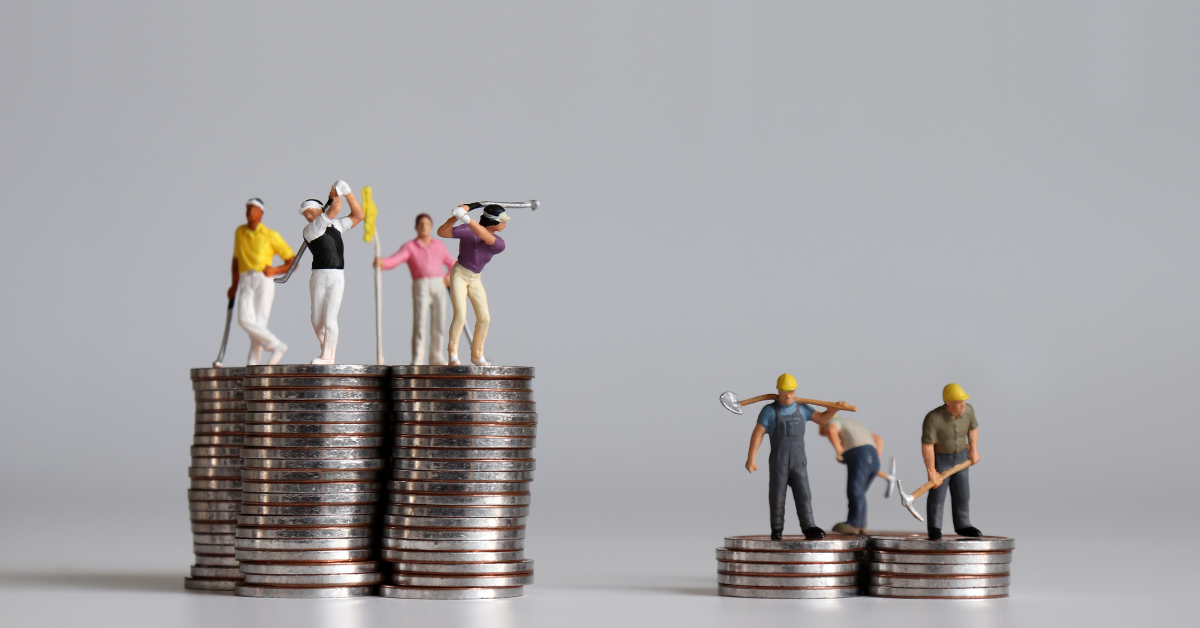
\includegraphics{exam_answers_files/mediabag/Rich-vs-Poor.png}

}

\caption{hermanes}

\end{figure}%

Formalmente, la correlación de ingresos entre hermanes se define como
sigue:

\[
\rho = \frac{\sigma^2_{\text{entre}}}{\sigma^2_{\text{entre}} + \sigma^2_{\text{dentro}}}
\]

donde:

\begin{itemize}
\item
  \(\sigma^2_{\text{entre}}\) es la \textbf{varianza entre familias}, es
  decir, la parte de la desigualdad en ingresos que se debe a
  diferencias sistemáticas entre familias,
\item
  \(\sigma^2_{\text{dentro}}\) es la \textbf{varianza dentro de las
  familias}, es decir, la desigualdad en ingresos entre hermanes de una
  misma familia.
\end{itemize}

\textbf{Respuesta:}

La correlación de ingresos entre hermanes mide cuánto se parecen los
ingresos de les hermanes entre sí. Es un indicador de cuánto influye el
origen familiar sobre los resultados económicos individuales.

\begin{itemize}
\item
  Si \(\rho \approx 1\), entonces toda la desigualdad se explica por
  diferencias entre familias. En la imagen, esto se vería como pilas de
  monedas de igual altura dentro de cada familia, pero alturas muy
  distintas entre familias. En este caso, la movilidad social es baja o
  nula.
\item
  Si \(\rho \approx 0\), entonces la mayoría de la desigualdad ocurre
  dentro de las familias: les hermanes pueden terminar con ingresos muy
  distintos, independientemente del origen familiar. En la imagen, las
  pilas de monedas dentro de una familia tendrían alturas muy distintas,
  y se parecerían a las pilas de otras familias. En este caso, la
  movilidad social es alta.
\end{itemize}

La correlación entre hermanes captura cuánto importa la suerte de nacer
en una familia específica. Si los ingresos de les hermanes son muy
similares (alta correlación), entonces el contexto familiar es
determinante. Esto refleja una estructura social rígida, con baja
movilidad social. Por el contrario, una baja correlación sugiere que,
incluso dentro de una misma familia, existen trayectorias muy diversas,
lo cual es consistente con una sociedad de alta movilidad, donde
factores individuales, oportunidades externas o decisiones personales
influyen más que el origen familiar.

\section{Parte II: Aplicación de
conceptos}\label{parte-ii-aplicaciuxf3n-de-conceptos}

A continuación se presentan los ingresos anuales (en miles de pesos) de
4 familias a lo largo de dos generaciones: padres/madres (Generación 1)
e hijos/as (Generación 2).

\begin{longtable}[t]{ccc}
\caption{Tabla de ingresos}\\
\toprule
\cellcolor[HTML]{2C3E50}{\textcolor{white}{\textbf{Familia}}} & \cellcolor[HTML]{2C3E50}{\textcolor{white}{\textbf{Ingreso Gen 1 (mil pesos)}}} & \cellcolor[HTML]{2C3E50}{\textcolor{white}{\textbf{Ingreso Gen 2 (mil pesos)}}}\\
\midrule
A & 100 & 50\\
B & 250 & 200\\
C & 500 & 600\\
D & 950 & 1550\\
\bottomrule
\end{longtable}

\subsection{Pobreza}\label{pobreza}

\subsubsection{Usando una línea de pobreza de 300 mil pesos per cápita,
calcula la tasa de pobreza en cada
generación.}\label{usando-una-luxednea-de-pobreza-de-300-mil-pesos-per-cuxe1pita-calcula-la-tasa-de-pobreza-en-cada-generaciuxf3n.}

\textbf{Respuesta:}

\[\text{Tasa de pobreza} = \frac{\text{número de personas con ingreso} < 300}{4}\]

\begin{itemize}
\item
  \textbf{Generación 1}: Las personas A y B tienen ingresos de 100 y 250
  mil pesos, respectivamente, ubicándolas bajo la línea de pobreza. Las
  personas C y D tienen ingresos superiores a 300 mil pesos. Por tanto,
  la asa de pobreza en Gen 1 es: \(\frac{2}{4} = 0.5\) (50\%).
\item
  \textbf{Generación 2}: Las personas A y B tienen ingresos de 50 y 200
  mil pesos, respectivamente, manteniéndolas bajo la línea de pobreza.
  Las personas C y D superan el umbral de 300 mil pesos. Por tanto, la
  asa de pobreza en Gen 2 es: \(\frac{2}{4} = 0.5\) (50\%).
\end{itemize}

\subsection{Desigualdad}\label{desigualdad}

\subsubsection{\texorpdfstring{Calcula el \emph{índice de Gini} y el
\emph{ratio entre el 25\% más rico y el 25\% más pobre} para cada
generación.}{Calcula el índice de Gini y el ratio entre el 25\% más rico y el 25\% más pobre para cada generación.}}\label{calcula-el-uxedndice-de-gini-y-el-ratio-entre-el-25-muxe1s-rico-y-el-25-muxe1s-pobre-para-cada-generaciuxf3n.}

Para aproximar el coeficiente de Gini utiliza la siguiente fórmula:

\[G = \frac{\sum_{i=1}^{n} \sum_{j=1}^{n} |y_i - y_j|}{2n^2 \bar{y}}\]

Donde:

\begin{itemize}
\item
  \(G\) es el índice de Gini, que mide la desigualdad. Su valor oscila
  entre 0 y 1.
\item
  \(\sum_{i=1}^{n} \sum_{j=1}^{n} |y_i - y_j|\) es la suma de las
  diferencias absolutas entre los ingresos.
\item
  \(n\) es el número de personas en la sociedad. En este caso,
  \(n = 4\).
\item
  \(\bar{y}\) es el ingreso promedio de la sociedad.
\end{itemize}

\textbf{Respuesta:}

Cálculo de Gini Gen 1:

\begin{itemize}
\item
  \(\bar{y} = \frac{100 + 250 + 500 + 950}{4} = 450\) mil pesos
\item
  \(\sum |y_i - y_j| = |100 - 250| + |100 - 500| + |100 - 950| + |250 - 500| + |250 - 950| + |500 - 950|\)
\item
  \(\sum |y_i - y_j| = 150 + 400 + 850 + 250 + 700 + 450 = 2.700\) mil
  pesos
\end{itemize}

El índice de Gini para la \textbf{Generación 1} es:

\[G = \frac{2.700}{2 \times 4^2 \times 450} = \frac{2.700}{2 \times 16 \times 450} = \frac{2.700}{14.400} = 0.4875 \approx 0.49\]

Cálculo de Gini Gen 2:

\begin{itemize}
\item
  \(\bar{y} = \frac{50 + 200 + 600 + 1550}{4} = 600\) mil pesos
\item
  \(\sum |y_i - y_j| = |50 - 200| + |50 - 600| + |50 - 1550| + |200 - 600| + |200 - 1550| + |600 - 1550|\)
\item
  \(\sum |y_i - y_j| = 150 + 550 + 1500 + 400 + 1350 + 950 = 4.900\) mil
  pesos
\end{itemize}

El índice de Gini para la \textbf{Generación 2} es:

\[G = \frac{4.900}{2 \times 4^2 \times 600} = \frac{4.900}{2 \times 16 \times 600} = \frac{4.900}{19.200} = 0.5104 \approx 0.51\]

Calculo el ratio entre el 25\% más rico y el 25\% más pobre en cada
generación:

\[\text{Ratio} = \frac{\text{Ingreso más alto}}{\text{Ingreso más bajo}}\]

\begin{itemize}
\item
  \textbf{Generación 1}: Ratio \(= \frac{950}{100} = 9.5\)
\item
  \textbf{Generación 2}: Ratio \(= \frac{1550}{50} = 31\)
\end{itemize}

\subsubsection{¿Qué nos enseñan ambas medidas sobre la desigualdad en
cada generación? Discute los resultados considerando ambas métricas.
¿Por qué podrían ofrecer diagnósticos distintos sobre la
desigualdad?}\label{quuxe9-nos-enseuxf1an-ambas-medidas-sobre-la-desigualdad-en-cada-generaciuxf3n-discute-los-resultados-considerando-ambas-muxe9tricas.-por-quuxe9-podruxedan-ofrecer-diagnuxf3sticos-distintos-sobre-la-desigualdad}

\textbf{Respuesta:}

Ambas medidas buscan capturar el grado de desigualdad en la distribución
del ingreso, pero lo hacen desde perspectivas distintas, por lo que
pueden ofrecer diagnósticos complementarios o incluso divergentes. En
este caso,

\begin{itemize}
\tightlist
\item
  \textbf{Gini}:

  \begin{itemize}
  \tightlist
  \item
    Generación 1: \(G = 0.49\)
  \item
    Generación 2: \(G = 0.51\)
  \end{itemize}
\item
  \textbf{Ratio entre extremos}:

  \begin{itemize}
  \tightlist
  \item
    Generación 1: \(\frac{950}{100} = 9.5\)
  \item
    Generación 2: \(\frac{1550}{50} = 31\)
  \end{itemize}
\end{itemize}

El índice de Gini considera todas las diferencias entre todos los pares
de ingresos, por lo que ofrece una medida global de la desigualdad. Es
más sensibles a cambios en la parte media de la distribución de
ingresos, pero menos sensible a cambios en los extremos. En cambio, el
ratio entre extremos sólo compara dos puntospor tanto es sensible a
cambios en los extremos de la distribución, pero ignora lo que pasa con
el resto de la población.

En este caso se observa que el Gini prácticamente no cambia pero hay
aumento dramático del ratio (de 9.5 a 31), indicando que la
concentración del ingreso en el extremo superior creció mucho más rápido
que la mejora de los ingresos en otros sectores.

\subsection{Movilidad intergeneracional del
ingresos}\label{movilidad-intergeneracional-del-ingresos}

\subsubsection{Calcula el porcentaje de movilidad absoluta ascendente y
descendente en cada
generación.}\label{calcula-el-porcentaje-de-movilidad-absoluta-ascendente-y-descendente-en-cada-generaciuxf3n.}

\textbf{Respuesta:}

\begin{itemize}
\item
  \textbf{Movilidad ascendente}: Las personas C y D aumentaron sus
  ingresos (de 500 a 600 y de 950 a 1550 mil pesos, respectivamente).
\item
  \textbf{Movilidad descendente}: Las personas A y B disminuyeron sus
  ingresos (de 100 a 50 y de 250 a 200 mil pesos, respectivamente).
\item
  \textbf{\% movilidad ascendente}: \(\frac{2}{4} = 0.5\) (50\%).
\item
  \textbf{\% movilidad descendente}: \(\frac{2}{4} = 0.5\) (50\%).
\end{itemize}

\subsubsection{Calcula la elasticidad intergeneracional de ingresos
(IGE), explica qué mide y discute su magnitud en perspectiva
internacional, con base en las lecturas de Corak y
Torche.}\label{calcula-la-elasticidad-intergeneracional-de-ingresos-ige-explica-quuxe9-mide-y-discute-su-magnitud-en-perspectiva-internacional-con-base-en-las-lecturas-de-corak-y-torche.}

Para ello, usa la siguiente fórmula:

\[\text{Elasticidad} = \frac{\text{Cov}(x, y)}{\text{Var}(x)}\]

donde las siguientes cantidades resumen la información contenida en los
datos de ingreso tranformados a logaritmo en base 10.

\begin{itemize}
\tightlist
\item
  \(\bar{x} = 2.52\), \(\bar{y} = 2.49\)
\item
  \(\text{Var}(x) = 0.174\), \(\text{Cov}(x, y) = 0.087\)
\end{itemize}

datos:

\begin{longtable*}[t]{ccc}
\toprule
\cellcolor[HTML]{2C3E50}{\textcolor{white}{\textbf{Persona}}} & \cellcolor[HTML]{2C3E50}{\textcolor{white}{\textbf{log Gen 1 (x)}}} & \cellcolor[HTML]{2C3E50}{\textcolor{white}{\textbf{log Gen 2 (y)}}}\\
\midrule
A & 2.00 & 1.70\\
B & 2.40 & 2.30\\
C & 2.70 & 2.78\\
D & 2.98 & 3.19\\
\bottomrule
\end{longtable*}

\textbf{Respuesta:}

\[
\text{Elasticidad} = \frac{0.087}{0.174} = 0.5
\]

Una elasticidad de \textbf{0.5} indica que el 50\% de las diferencias
relativas en ingresos entre padres y madres se transmiten a sus hijos e
hijas. En otras palabras, las personas cuyos padres tienen ingresos
altos tienden a tener ingresos altos también, y viceversa.

Según Corak, las sociedades con alta elasticidad (por sobre 0.4) se
caracterizan por una baja movilidad intergeneracional y una fuerte
reproducción de las desigualdades económicas. Este valor ubicaría a esta
sociedad hipotética en un nivel de movilidad similar al de países con
alta desigualdad y baja movilidad como Estados Unidos. En contraste,
países como Dinamarca, Canadá o Noruega muestran elasticidades entre
0.15 y 0.2, lo que refleja mayores oportunidades de movilidad económica.

Como señala Torche, una elasticidad de 0.5 no solo refleja que los
ingresos se heredan parcialmente, sino también que las instituciones
sociales y económicas amplifican las ventajas iniciales. Este resultado
es consistente con una estructura social en la que las oportunidades
están fuertemente condicionadas por el origen familiar.

\section{Parte III: Discusión}\label{parte-iii-discusiuxf3n}

Considerando todos los resultados obtenidos en la Parte II,

\subsubsection{Caracteriza y compara ambas generaciones en términos de
sus niveles y patrones de pobreza, desigualdad y
movilidad.}\label{caracteriza-y-compara-ambas-generaciones-en-tuxe9rminos-de-sus-niveles-y-patrones-de-pobreza-desigualdad-y-movilidad.}

Para responder a esta pregunta no olvides referirte los siguientes
conceptos (si corresponde):

\begin{itemize}
\tightlist
\item
  pobreza absoluta y pobreza relativa
\item
  distribución del ingreso
\item
  movilidad absoluta y movilidad relativa
\end{itemize}

\textbf{Respuesta:}

\begin{itemize}
\item
  No hay reducción de la pobreza absoluta entre generaciones.
\item
  Hay un leve aumento en el ingreso promedio y estabilidad de la
  desigualdad global (según Gini).
\item
  Se observa un fuerte crecimiento en la distancia entre ricos y pobres
  (según ratio).
\item
  Hay movilidad absoluta en ambas direcciones pero la movilidad relativa
  es baja.
\end{itemize}

En conjunto, esto indica una sociedad con crecimiento económico desigual
y persistencia estructural de las desventaja.

\subsubsection{Considerando la descomposición de Datt-Ravallion, ¿cómo
podría reducirse la pobreza en la Generación 2 si se descarta el
crecimiento económico como opción? Explica tu
respuesta.}\label{considerando-la-descomposiciuxf3n-de-datt-ravallion-cuxf3mo-podruxeda-reducirse-la-pobreza-en-la-generaciuxf3n-2-si-se-descarta-el-crecimiento-econuxf3mico-como-opciuxf3n-explica-tu-respuesta.}

\textbf{Respuesta:}

Si el crecimiento económico no es una opción, la reducción de la pobreza
debe apoyarse en políticas de redistribución. En esta sociedad
hipotética, reducir la concentración de ingresos en el extremo superior
(como se refleja en el ratio 31) podría liberar recursos para mejorar
los ingresos de quienes están bajo la línea de pobreza. Por ejemplo,
políticas fiscales redistributivas o transferencias directas podrían
mejorar los ingresos reales de los hogares pobres, incluso sin aumentar
el ingreso nacional total.

\begin{tcolorbox}[enhanced jigsaw, colbacktitle=quarto-callout-tip-color!10!white, colback=white, rightrule=.15mm, toprule=.15mm, coltitle=black, bottomtitle=1mm, toptitle=1mm, opacityback=0, leftrule=.75mm, breakable, title=\textcolor{quarto-callout-tip-color}{\faLightbulb}\hspace{0.5em}{Fin del examen}, colframe=quarto-callout-tip-color-frame, opacitybacktitle=0.6, bottomrule=.15mm, titlerule=0mm, arc=.35mm, left=2mm]

Revisa tus respuestas antes de entregar.

\end{tcolorbox}




\end{document}
